\documentclass[aspectratio=169]{beamer}

\usetheme{vega}

\title{Report on my research}
\subtitle{SRG Market microstructure}
\author{Vsevolod Zaostrovsky}
\institute{Vega Institute Foundation}
\supervisor{Anton Belyakov, Alexey Savin}
% \date{August 21 -- 28, 2022}

\usepackage[]{lipsum}
\begin{document}
\maketitle

\begin{frame}{Our methodology to fit parameters $\rho, \kappa, q$}
    We chose regression to find parameters:                                                                                                                                                                                                                                                                                                                                                                                       
            \begin{equation*}
                \frac{\Delta A_{k+2}}{\Delta t_{k+2}} - \frac{\Delta A_{k+1}}{\Delta t_{k+1}} 
        = - \rho \Delta A_{k+1} + \rho \lambda x_{k+1} + (\kappa + \lambda) (\frac{x_{k+2}}{\Delta t_{k+2}} - \frac{x_{k+1}}{\Delta t_{k+1}}).
            \end{equation*}

        Where all the information needed can be extracted from the l3 data: 
        \begin{itemize}
            \item $\Delta A_{k}$ is an ask change after execution of the limit order with the depth $x_k$.
            So, $\Delta A_{k} = \textrm{AskAfter}(k) - \textrm{AskBefore}(k)$ and $x_k = \textrm{Volume}(k)$.
            \item $\Delta t_{k}$ is a time between $k$ and $k + 1$ orders of dataset. So, $\Delta t_{k} = \textrm{Time}(k+1) - \textrm{Time}(k)$
        \end{itemize}
\end{frame}

\begin{frame}{Backtest methodology}
    According the OW model, ask dynamics should follow the equation:
    \begin{equation*}
        A_t = \overline p _t + \frac{s}{2} + x_1 \kappa e^{- \rho t},
    \end{equation*}
    where $A_t$ --- ask price after execution, $\overline p _t + \frac{s}{2}$ defines steady state level 
    (here $\overline p _t$ is a price and $s$ is a spread), $\kappa$ and $\rho$ are hyperparameters. \par
    Important details:
    \begin{itemize}
        \item According the paper, $\kappa > 0$, $\rho > 0$. 
        \item From \href{https://www.desmos.com/calculator?lang=ru}{numerical properties} of the function:
        \begin{itemize}
            \item $A_t$ can be $1-2$ more then $V_t$ not 100, so $|\kappa| << 1$. 
            \item $\rho$ should not be too big (about $10000$, for example), because in this case, resilency should be so huge, so all 
            execution strategies are useless: you can just sell as many stocks as you want.
        \end{itemize}
    \end{itemize}
\end{frame}

\begin{frame}{Problems}

    \begin{itemize}
        \item In all the tests $\rho > 1000$ and $\kappa < 0$, so we get useless parameters. 
        \item One can say that problem can be fixed by considering $t$ in ms instead of seconds, but it had not work.
        \item I don't emperically observe such dynamics:
        \begin{figure}
            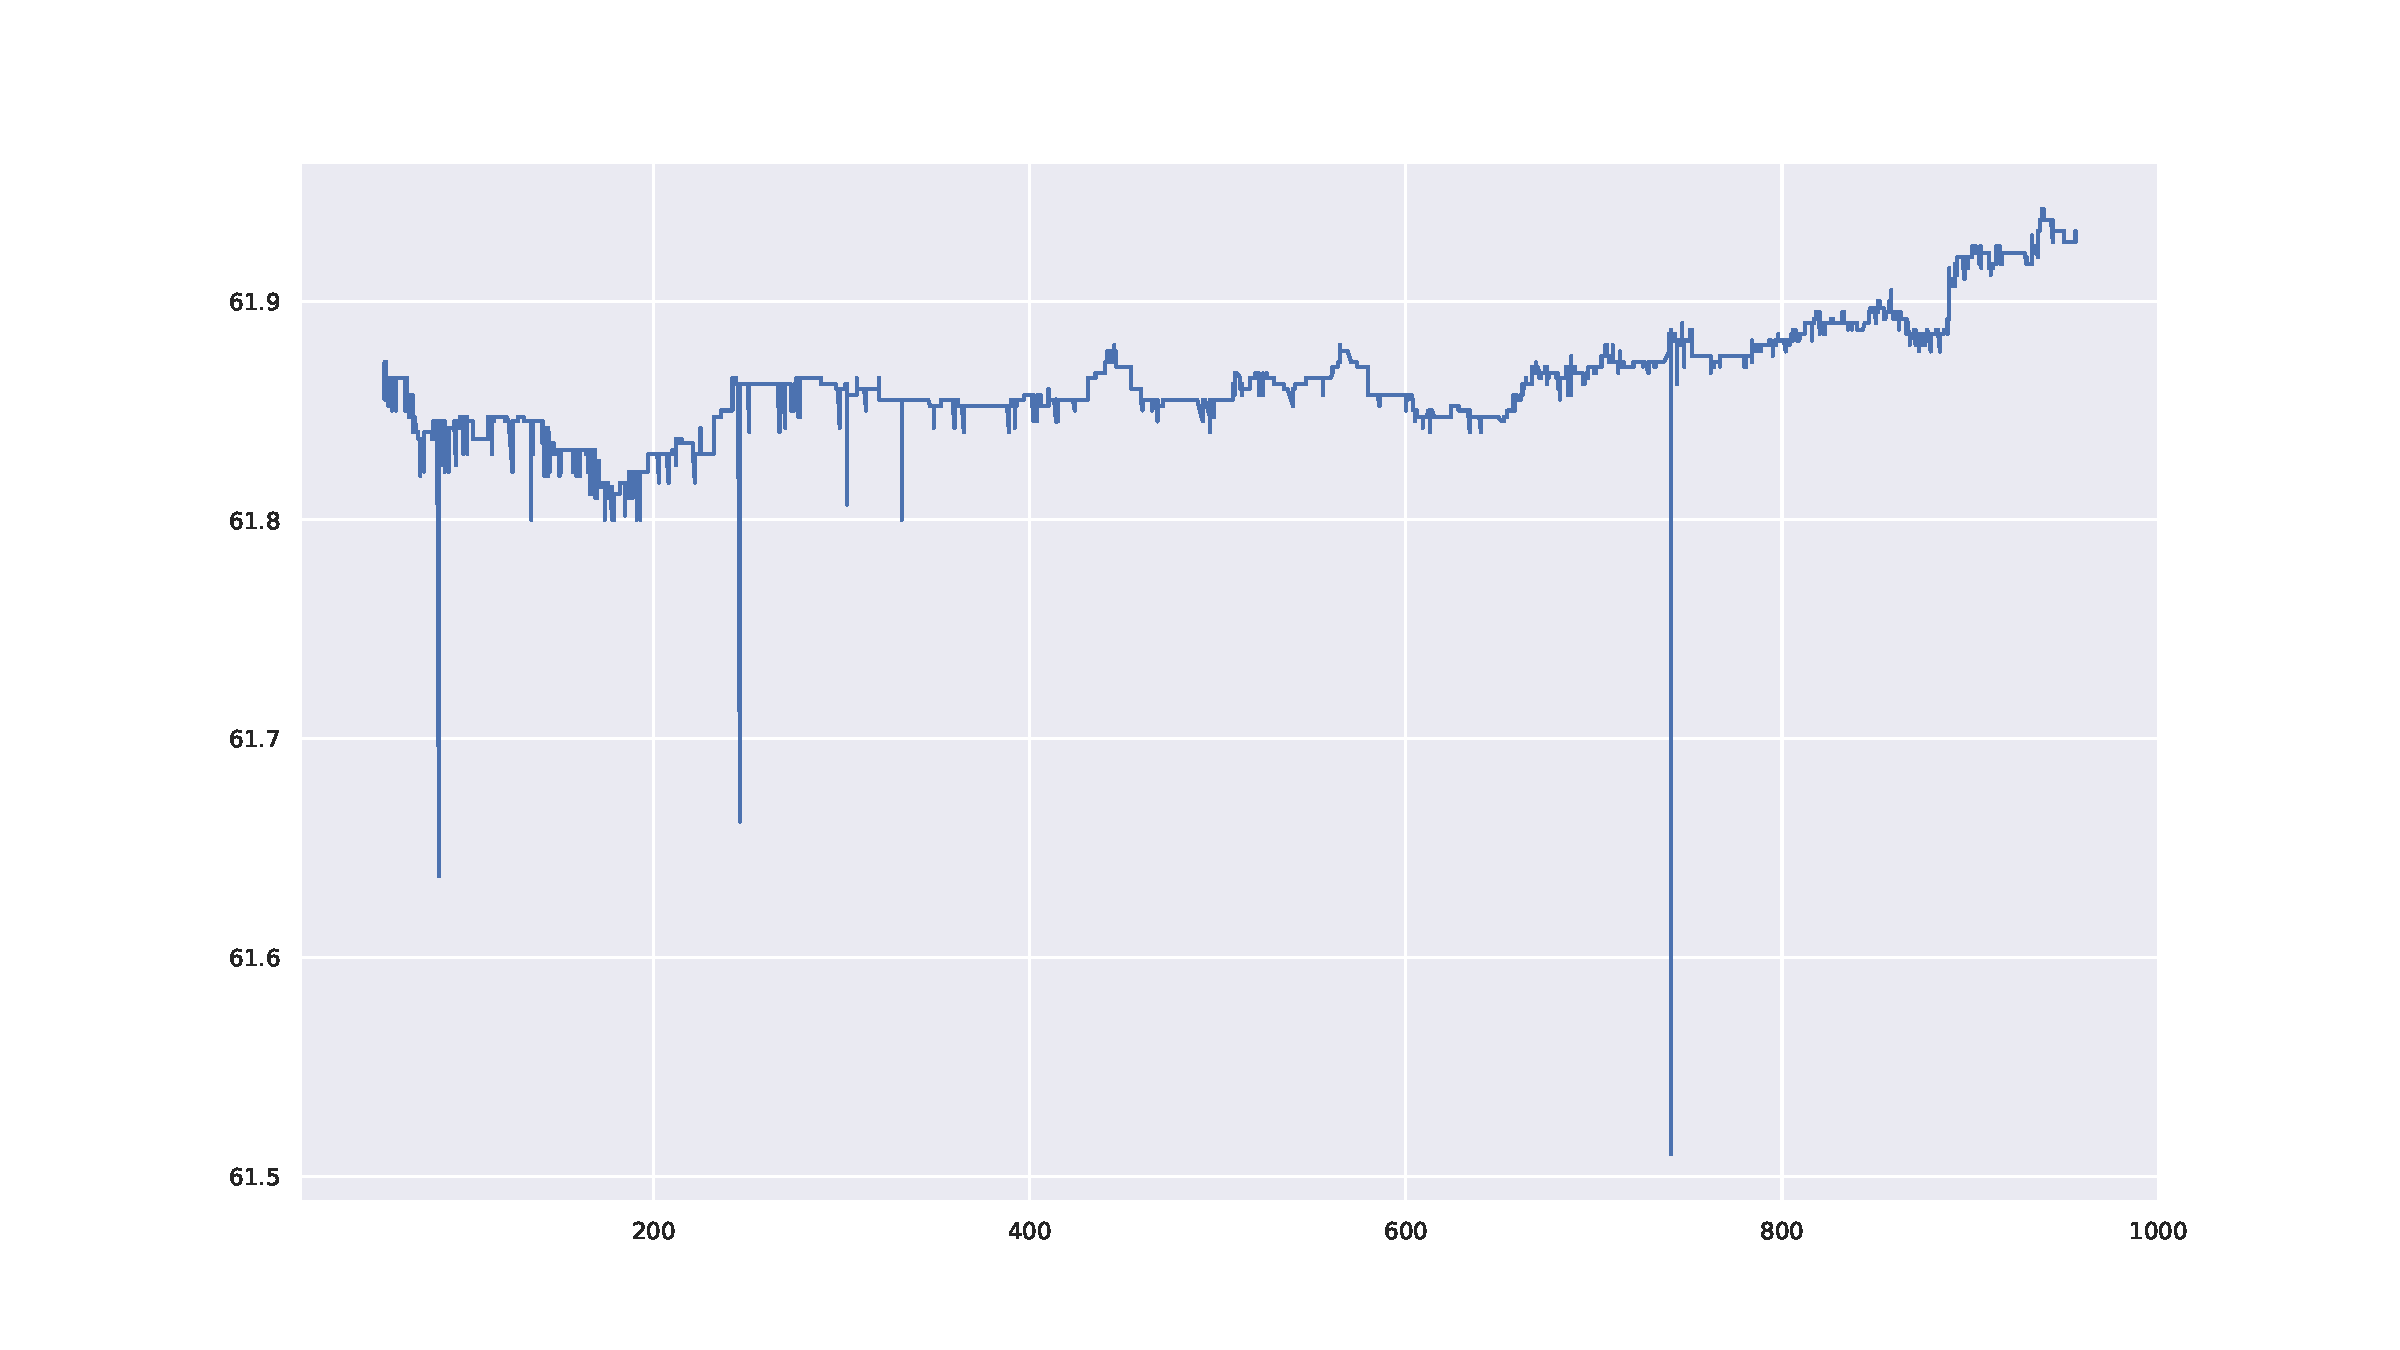
\includegraphics[scale=0.25]{figs/AsksHistory.pdf}
            \caption{Asks history}
            \label{fig:mvslim}
        \end{figure}
    \end{itemize}
\end{frame}

\begin{frame}{Another approach to fit the parametrs.}
    According the OW model, ask dynamics should follow the equation:
    \begin{equation*}
        A_t = \overline p _t + \frac{s}{2} + x_1 \kappa e^{- \rho t},
    \end{equation*}
    so lets try to use OLS to fit the parameters according the ask dynamics. As a steady state level we will consider ask before the execution, so we get:
    \begin{equation*}
        \textrm{AskAfter}(k) = \textrm{AskBefore}(k) + \textrm{Volume}(k) \kappa e^{- \rho \textrm{Time}(k)}.
    \end{equation*}
\end{frame}


\end{document}